\chapter{Detailed Description}
\section{Interpreter}
\subsection{Introduction}
The interpreter is a complete implementation of an interpreter for the -{}-C language. It accepts input from the parser in the form of an AST (\emph{Abstract Syntax Tree}) and obeys the instructions contained within the nodes of the tree. We call the tree traversal ``a tree walk" and we use this walk to interpret \verb!NODE! terms on the fly. We will see this kind of recursive pattern several times throughout the whole project.
\subsection{Initial Scan}
Firstly, the interpreter scans the AST, looking for global variables and function definitions. This initial scan is done, as we have no idea where to start interpreting without the presence of some kind of entry point into the user's code. It was decided that the most sensible approach would be to require the user-supplied definition of an \verb!int main(void)! entry-point function, in a similar vain to C. As this initial sweep of the AST takes place, any global variables or function declarations are entered into a structure known as the ``environment". 
\subsection{Environment}
Quite simply, the environment houses everything that the interpreter considers to be in local scope at a given execution point. As such, after our initial scan, we can detect the presence of a valid entry-point function by examining the environment. This initial environment is known as the ``global environment", as everything contained within, is visible to the whole user programme. This initial scan follows exactly the same code-path as the full interpreter does, but passes a flag, in order to ensure that function bodies are never stepped into.
\ \\ \ \\
The environment (depicted in figure \ref{fig:environment}) is a hash-table of \verb!values!. These values are references to inner functions or local variables. By following the static link between one environment and another (please see figure \ref{fig:environment}), it is possible to access and refer to values residing in outer scopes. The idea of a static link was given to us in relation to their use in Activation Records (please see section \ref{section:MIPS}) during lectures. Different information is stored for functions as opposed to variables. The \verb!value!'s type is determined with the following constants, the main types are given here, although there are some used for other purposes that are not mentioned here for the sake of clarity.

\begin{description}
	\item[VT\_INTEGR] Values of this type are integer variables, integer constants or integer temporaries.
	\item[VT\_STRING] Strings cannot be stored in the environment (this language does not have a string type), this value type is used to construct temporary strings that can be passed around within the interpreter / compiler. Such string values are created when identifiers are walked over, for instance.
	\item[VT\_FUNCTN] These values represent pointers to functions. This can be either a function variable or an actual function.
\end{description}

\subsection{Invoking the entry point}
If no entry point is found, a fatal error is raised as interpretation cannot continue without a valid entry point. If the entry point was found in our global environment, we lookup where the function definition was found in the AST and execute from this point. The \verb!environment.c! file gives us lots of useful search functionality in order to do things such as this. The particular search we do to find the main entry point is to look for a function in the global environment called \verb!main! with an integer return type and no formal parameters. If we get a match, we are returned a \verb!value! structure (of type \verb!VT_FUNCTN!) which meets our requirements within the global environment. These ``function values" each hold a reference to what \verb!NODE! in the AST is considered the ``start of the function". Once we have found the corresponding ``start of function" \verb!NODE! for the \verb!main()! function, we are able to continue the interpretation process by calling \verb!evaluate! on this entry \verb!NODE!.

\subsection{Main recursive function - evaluate()}
The \verb!evaluate! function is now called recursively starting from the entry point. This scan is different from the initial scan, because we now look inside function bodies and any nested functions contained therein. Every time we enter a new function or block (such as an \emph{if statement} or \emph{while loop}), a new environment is created with a static link to the environment of the parent (enclosing) function (or the global environment, as appropriate). As we step over the tree in this recursive function, we encounter \verb!NODES! that are present in the AST. The following list mentions the steps that are taken for the several different (more interesting) types of node. The terms LHS and RHS refer to the \emph{left-hand side} and \emph{right-hand side} of an expression respectively. As the AST is a binary tree, the LHS and RHS can be thought of as the two child nodes under the current node. Please see figure \ref{fig:ast} for an example AST, that will use some of the elements mentioned below.

\begin{description}
	\item[Arithmetic Operator] We look at the LHS and RHS of the expression call \verb!evaluate! recursively on each. We do this, to try and simplify both sides (operands) into integers. From each recursive call we get back a \verb!value! typed struct for each, which should now contain our simplified integer. If one side happened to be a function application, for instance, the recursive call has already made the necessary calls to coerce this into the appropriate integer value. We calculate the result of the arithmetic expression and return the calculated value.
	\item[= Operator] This is the assignment operator. We call \verb!evaluate! on the LHS to get the variable into which the result will be stored. For the assignment to be valid, we must have already defined the assignment variable in the environment. Otherwise, we would be  using a variable that has not been declared yet. We call \verb!evaluate! on the RHS to find out the value that we're trying to assign to the variable on the LHS. Once we have the value back, we \textbf{type check} the assignment to ensure that the assignment is valid. This prevents the user making mistakes like trying to assign an integer to a function typed variable. The type checking operation is a simple check on the \verb!value! type on the LHS and RHS to check that they match. If the types do not match, then a fatal error describing the problem is raised. If all checks pass, then the existing LHS variable is updated with the new RHS value. This assignment will always affect the variable in the environment of its definition. The next time this LHS variable is referenced, it will have the newly assigned value.
	\item[APPLY] The \verb!APPLY! node type is encountered when a function call will occur. On the LHS of an \verb!APPLY! node is the function name identifier and the RHS contains the list of parameters that are being passed to the function. To invoke the function, the function name is searched for within the current environment (traversing static links where necessary). If the function is not found, a fatal interpreter error is raised. If the function is found, we switch to the function's definition environment. In this environment, we store new variables with the formal parameter names, but with the specified parameter values used when calling the function. This assignment is also type checked with precisely the same method as before (see point ``\textbf{= Operator}" above). Once the checks are complete, we now pass the AST node representing the start of the function body to the \verb!evaluate! function and wait for control to return with the associated return value.
	\item[WHILE] While loops are also possible in C-{}-. The implementation for a \verb!WHILE! statement within -{}-C actually relies on the \verb!while! construct in the host development language (C).
\end{description}


\begin{figure}[p]
	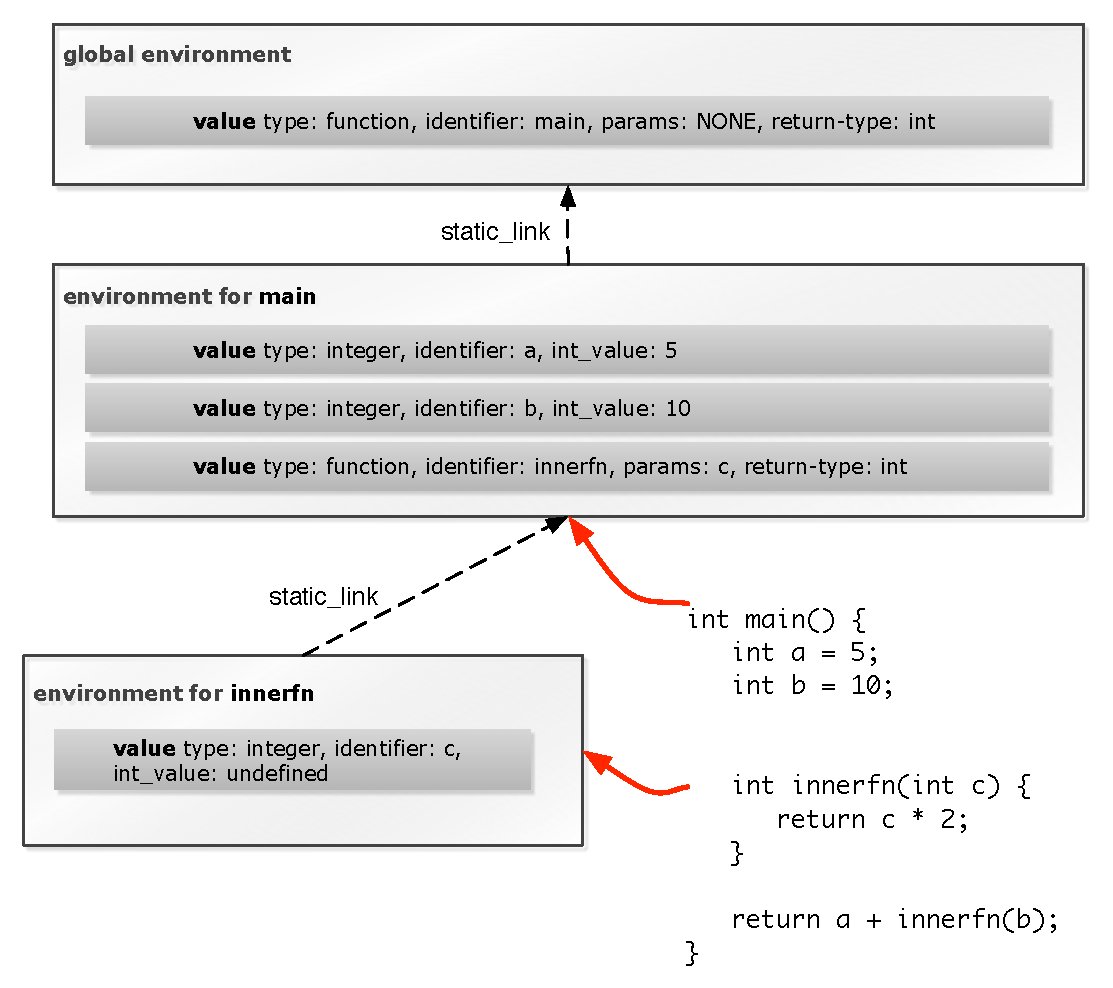
\includegraphics[scale=0.7]{environments-include.pdf}
	\caption{Environment Layout - Environment $\rightarrow$ Code relationship}
	\label{fig:environment}	
\end{figure}

\begin{figure}[p]
	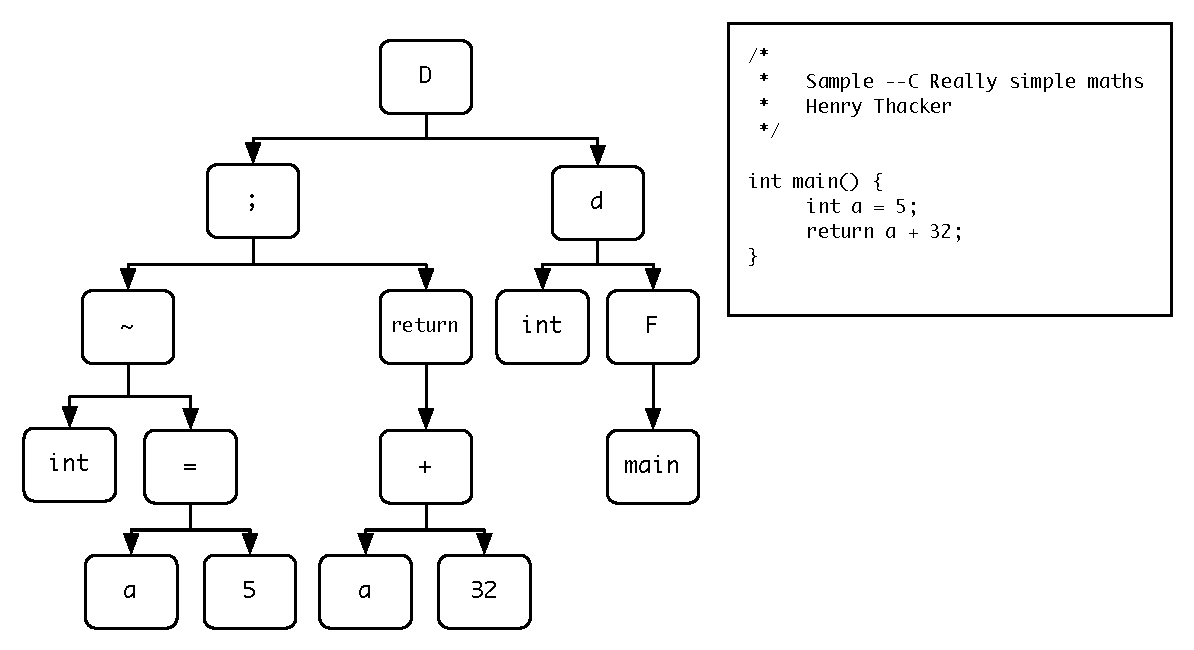
\includegraphics[scale=0.7]{ast-include.pdf}
	\caption{Abstract syntax tree example}
	\label{fig:ast}
\end{figure}


\section{Intermediate Representation}
\label{section:MIPS}
\section{MIPS Assembler Compiler}